
\documentclass[10pt,twocolumn]{witseiepaper}
%
% All KJN's macros and goodies (some shameless borrowing from SPL)
\usepackage{KJN}
\usepackage{rotating}
\usepackage{tikz}
\usepackage[super]{nth}
\usepackage{subcaption}
\usepackage{listings}
\usepackage{lscape}
\usepackage{amsmath}
\usepackage{epstopdf}
\usepackage{xcolor}
\usepackage{textcomp}
\usepackage{listings}
\usepackage{alltt}
%\usepackage{matlab-prettifier}
\usepackage{graphicx}
\usepackage{changes}
\usepackage{makecell}
\usepackage{verbatim}
\usepackage{algorithm,algpseudocode}
\usepackage{balance}
\usepackage{pdfpages}
\usepackage{makecell}
\usepackage{color} %red, green, blue, yellow, cyan, magenta, black, white
\definecolor{mygreen}{RGB}{28,172,0} % color values Red, Green, Blue
\definecolor{mylilas}{RGB}{170,55,241}
%\usepackage{flafter}
\usepackage{tikz}
\usetikzlibrary{shapes,arrows}
\usepackage[utf8]{inputenc}
\usepackage[english]{babel}
\usepackage{pgfgantt}
\newcommand\Tstrut{\rule{0pt}{2.2ex}} 
\usepackage{float}
\usetikzlibrary{matrix,chains,positioning,decorations.pathreplacing,arrows}
\usetikzlibrary{decorations.text}
\usetikzlibrary{decorations.pathmorphing}
\usetikzlibrary{fit, arrows.meta}
\usetikzlibrary{shadows,trees}
\lstset{language=Matlab, % Set colour for matlab code
	breaklines=true,%
	morekeywords={matlab2tikz},
	keywordstyle=\color{blue},%
	morekeywords=[2]{1}, keywordstyle=[2]{\color{black}},
	identifierstyle=\color{black},%
	stringstyle=\color{mylilas},
	commentstyle=\color{mygreen},%
	showstringspaces=false,%without this there will be a symbol in the places where there is a space
	numbers=left,%
	numberstyle={\tiny \color{black}},% size of the numbers
	numbersep=9pt, % this defines how far the numbers are from the text
	emph=[1]{for,end,break},emphstyle=[1]\color{red}, %some words to emphasise
	%emph=[2]{word1,word2}, emphstyle=[2]{style},    
}
%
% PDF Info
%
% correct bad hyphenation here
\hyphenation{op-tical net-works semi-conduc-tor}


\begin{document}
\title{ELEN4012 - EMOTION RECOGNITION PROJECT PLAN}

\author{Sasha Berkowitz (818737) \& Arunima Pathania (1117426)
	\thanks{School of Electrical \& Information Engineering, University of the
		Witwatersrand, Private Bag 3, 2050, Johannesburg, South Africa}
}
	
\abstract{The plan for the design and development of a speech emotion recognition classifier is presented. The system is to recognise happiness, sadness, anger and fear in 2~second inputs from English and Afrikaans speakers. This will be done through enhancing a signal with the NPVSS-NLMS, GSVSS-NLMS, RLS and Affine Projection filters, converting them to MFCC spectrograms and using MLP and CNN classifiers. A simple user interface will be developed and all will be carried out using the Python language, as well as Google's TensorFlow library for machine learning aspects. Success will be achieved if the system has an accuracy of 50 \% or above. The project's work breakdown has been provided along with inherent risks and their mitigations, as well as socio-economic considerations. }

\keywords{artificial intelligence, convolutional neural network, emotion recognition, multilayer perceptron, signal enhancement,MFCC.}

	\maketitle
	
	\vspace{7pt}
\section{Introduction}
Emotion detection from speech is a process that deals with discovering the emotional aspect of speech irregardless of the speech content. This feature would help in providing better services as the machine would be adaptive to human emotion, resulting in a more realistic human-machine interaction. The aim of the project is thus to develop in a system that can detect speech emotion for English and Afrikaans language speakers.

The project employs use of speech enhancement and classification in order to achieve more desirable results.
It will also make use of four filters as speech enhancement schemes, namely:  Non-parametric variable step size normalised least mean square (NPVSS-NLMS) algorithm, Generalised sigmoid variable step size normalised least mean square (GSVSS-NLMS) algorithm, Normalised lattice recursive least squares filter (NLRLS) algorithm and the fast affine projection algorithm. The speech classification is implemented by neural network algorithms such as Multilayer Perceptron (MLP) and convolutional neural network (CNN).

This project attempts to clearly distinguish between the different emotions in human speech. It will also show comparative results of the developed system in cases where the speech enhancement scheme is absent, between the two languages employed and between the two different classifier algorithms used in order to find out which gives the greatest results.

Section~\ref{sec:lr} of this report explores previous solutions relevant to the given problem and section~\ref{sec:spec} the problem specifications. Sections~\ref{sec:approach} and \ref{sec:management} describe the proposed approach to be taken and how it will be split and managed, respectively. Section~\ref{sec:risks} lists the project risks and discusses mitigations put into place in order to avoid them and section~\ref{sec:social} describes its socio-economic effects. Finally, this report is concluded in section~\ref{sec:conc}.

\section{Literature Review}\label{sec:lr}
With the increase in the amount of readily available information in the modern world, as well as the vast, growing computational power at our disposal, popularity in the development of artificial intelligence and machine learning is on the rise. This technology is often used to mimic human-like decision making and judgements, such as understanding images and audio. The understanding of images and audio assist in simulating conversations and are useful in cases where chatbots can replace human assistants~\cite{chatbot}. In addition to the recognition of spoken words, a new aspect that can be added to these bots is emotional recognition to help them with understanding the human they are conversing with.
\hfill\\

For complex problems, such as an automatic emotion recognition in  speech, a neural network (NN) is suitable. NNs are part of the representation learning algorithm class, where large and complex problems are broken down into smaller ones, making them more manageable~\cite{tensorIntro}. Within the neural network class, multiple architectures exist and it is important to choose one well suited for a given project.

These NNs, as described above, require precise and valuable data in order to train the network - a process where the network model is fed a large number of sample input cases and their expected outputs in order to 'teach' it how to think for itself~\cite{tensorIntro}. In the case of a speech signal input, often there is unwanted noise present affecting the quality of the information fed into the network. It is therefore important to take steps to minimise the noise present and enhance the signal in the system design by making use of filtering.

Most popular NN architectures employed for audio recognition classifier are recursive neural networks (RNN), convolutional neural networks (CNN) and multi-layer perceptrons  (MLP). In the case of emotion recognition, a solution is offered by Ram et al. where fear is recognised in speech through the use of a MLP classifier and least mean square, normalised least mean square and recursive least mean square filters are applied to input signals~\cite{fearMLP}. This solution managed a 77\% accuracy in recognising fear in speech~\cite{fearMLP}. 

An important consideration to take on input data is its representation. In order for the NN, or classifier, to extract and analyse features from each input, the input should be in a form where it is suitable to do so. In order for audio signals to be represented meaningfully often a number of fast Fourier transforms are applied to it and its output frequencies mapped as an array or RGB image. An example of this is demonstrated by Stolar, et al. where real time emotional speech signals are separated into one second blocks, converted to spectrograms and then RGB images, before being analysed using a five convolutional layer CNN\cite{RGB}.

In order to further increase input quality, additional means of filtering acoustic echo are offered by Hamidia, et al. with an improved design on the variable step-size normalised least mean square (VSS-NLMS) algorithm, combining the generalised sigmoid variable step-size NLMS with the estimation error ratio~\cite{echo}.
\hfill\\

An ever-growing popular choice for building these neural networks is Google's open-source library, TensorFlow. TensorFlow (mainly implemented in the Python language) uses dataflow graphs with nodes representing mathematical operations and edges tensors - multidimensional arrays~\cite{tensorIntro}. Through the use of the tensor data representation, performing operations on large datasets has become a much more efficient practice. Additionally, the library has support for multiple CPUs and GPUs as well as cross-operating system support~\cite{tensorIntro}. For these reasons, developing neural networks using Python over tools such as Matlab has become well suited and increasingly user-friendly. 

%\vspace{7pt}
\section{Problem Specification}\label{sec:spec}
\subsection{Overview}
The aim of this project is to detect an emotion from input speech for a speaker of the English or Afrikaans languages. There are four proposed emotions that the researchers are working on namely, happiness, sadness, anger and fear. The study is intended to assist in the evolving field of artificial intelligence as it will create smarter systems to detect human emotion and enhance the interaction between human and machine. The contextualization section above shows how several methods have been implemented to detect emotion from speech. The main techniques used to perform this project include  signal enhancement using adaptive filters , feature extraction using the Mel Frequency Cepstral Coefficients (MFCC) and signal classification using neural network algorithms such as Multi-layer perceptrons  and the convolutional neural networks. The following points will motivate the usage of these techniques:
\subsubsection{Advantages}
\begin{itemize}
	\item Neural networks are highly accurate when identifying pattern recognition which includes speech recognition. 
	\item Neural networks have high computational power and therefore enable larger data sets to be processed 
	\item Adaptive filters change their filter parameters  to get accustomed to the change in signal characteristics in an unknown environment and hence work efficiently for noise cancellation.
	\item MFCC values give high accuracy in the frequency representation of speech signal.
\end{itemize}

\subsubsection{Disadvantages}
\begin{itemize}
	\item The biggest disadvantages of neural networks is the black box implementation since if something goes wrong you would not know how to fix it.
	\item  Machine Learning problems require very high amounts of data to obtain accurate results which can be very tedious.
	\item MFCC values are not robust and might need normalization when exposed to a noisy environment.
\end{itemize}
\subsection{Requirements}
Listed below are the major requirements for this project: 
\begin{itemize}
	\item The initial requirement entails finding the right algorithms for the signal enhancement and classification processes. 
	\item The designing and developing of the system which would recognize emotions from both English and Afrikaans.
	\item The system has to be trained and tested with large data sets of different emotions.
	\item To check the system operations it needs to be validated against a new set of data.
	\item A user interface is required for real-time application. 
\end{itemize}  

\subsection{Assumptions}
Listed below are the assumptions made for this project: 
\begin{itemize}
	\item The user is effectively able to communicate in either English or Afrikaans 
	\item The neural network would be able to differentiate between emotions with only a couple of thousand data points.
	\item The validation of the system will be performed in an environment of minimum background noise.
\end{itemize}  
\subsection{Constraints}
Listed below are the constraints faced during this project: 
\begin{itemize}
	\item The project has a deadline of six weeks.
	\item The data collection of the project can not be performed without ethical clearance from the University
	\item The noise cancellation filters do not give a 100\% accuracy and so the model will have to be trained with noise in the desired signal. 
	\item Changes in the natural state of voice will affect the system's accuracy i.e the speed of speech or the hoarseness of a voice.
\end{itemize}  
\subsection{Success Criteria}
Listed below are the success criterion of the project deliverable and management:
\begin{itemize}
	\item The project must meet all the requirements mentioned above while also adhering to the assumptions and constraints of the project.
	\item The project is expected to have an accuracy of above 50\%.
	\item The project should successfully be able to distinguish between all the specified emotions in human speech.
	\item The designed gantt chart should be followed and the desired work load division  should be met.
\end{itemize}



%~~~~~~~~~~~~~~~~~~~~~~~~~~~~~~~~~~~~~~~~~~~~~~~~~~~~~~~~~~~~~~~~~~~~~~~~~~~~~~~~~~~~~~~~~~
\section{Proposed Approach}\label{sec:approach}



\subsection{Approach Overview}
The task of building a system capable of recognising emotion from raw speech input has been separated into a few major subtasks to be performed. These tasks consist of recording an input signal, enhancing that signal through a number of filters, converting that signal into something that could provide meaning to the classifier, classifying the signal through a machine learning model and finally outputting an emotion and displaying it to a user. A breakdown of these tasks are shown in figure~\ref{fig:sysOverview} and their details will be discussed in sections~\ref{sec:si} through \ref{sec:traintest}.

\tikzstyle{block} = [draw, fill=white, rectangle, 
minimum height=3em, minimum width=3em]
\tikzstyle{sum} = [draw, fill=white, circle, node distance=1cm]
\tikzstyle{input} = [coordinate]
\tikzstyle{output} = [coordinate]
\tikzstyle{pinstyle} = [pin edge={to-,thin,black}]
\begin{figure*}[h]
	\centering
	\begin{tikzpicture}[auto, node distance=3.6cm,>=latex']
	\node [input, name=input] {};
	\node [block, right of=input,text width=2.2cm, text centered] (sensor) {Signal Enhancement};
	\node [block, right of=sensor,node distance=3cm, text width=1.7cm, text centered] (cond1) {Feature Extraction};
	\node [block, right of=cond1,node distance=3cm, text width=2.2cm, text centered] (cond2) {Signal Classification};
	\draw [->] (sensor) -- node[name=u] {$ $} (cond1);
	\draw [->] (cond1) -- node[name=v] {$ $} (cond2);
	\node [output, right of=cond2] (output) {};
	\coordinate [below of=u] (measurements) {};
	\draw [draw,->] (input) -- node {$Speech~Signal$} (sensor);
	\draw [->] (cond2) -- node [name=y] {$ Emotion$}(output);
	\end{tikzpicture}
	\caption{Block diagram of approach overview.}
	\label{fig:sysOverview}
\end{figure*}


\subsection{Speech Input}\label{sec:si}
Speech signals will be used as an input for both the training model as well as the final application. The inputs will be of a standard two second length, as implemented in~\cite{RGB}.

For the model training, speech will be sourced from recordings taken of students. These will be done in a soundproof chamber in order to reduce external interruption. In order to reduce project costs these will be done one of the project partners' iPhones which record at as M4A files, which will be converted to .WAV files for use. This will be done by using the built-in 'Voice Memo' application, which records at frequencies of 44.1 and 48~kHz~\cite{recordingFreq}.

In order to elicit emotions, students with an interest in drama or acting will be asked to participate and will be given an excerpt to read, along with an emotion to portray. This will be done in English as well as Afrikaans.

In addition to these recordings taken, sound files may be taken from online databases in order to strengthen the model's accuracy.

\subsection{Signal Enhancement}  \hfill\\
Signal enhancement refers to the refinement of an input signal to meet the requirements of a system for which the input is being used. This project requires an individual to speak into a microphone and the audio signal is then enhanced according to the needs of the project. 

As the audio signal will include background noise and channel distortion affecting the speech signal, the signal will be applied to a number of filters. These filters will remove any unwanted frequencies, therefore enhancing the signal to be analysed.

The human speech is typically made up of frequencies ranging from 300~Hz to 3~kHz. Limiting the signal to this frequency band through filtering will reject most part of the noise, as well as the plosive consonants like “p” and “t” which require a higher frequency to be correctly differentiated. This reason contributes to the selection of a higher frequency band which ranges over 300 Hz to 8 kHz[1]. 

As suggested by \cite{echo}, two variable step size adaptive filters will be used, being a non-parametric variable step size normalized least mean square (NPVSS-NLMS) algorithm ,a generalized sigmoid variable step size normalized least mean square (GSVSS-NLMS) algorithm and a Recursive least squares filter (RLS). In addition, a fast affine projection algorithm will be applied. These filters will be explained in sections~\ref{sec:af} through \ref{sec:affine}.

\subsubsection{Adaptive Filters}\label{sec:af} \hfill\\
An adaptive filter is a system with a linear filter which is self-designing and controlled by variable parameters. It uses a recursive algorithm to continuously adjust its tap weights to operate in new environments. It is made up of a digital filter and an algorithm designed to assist in adjusting the tap weights of the filter.  The microphone signal is represented by d(n). In the single-talk scenario, d(n) is made up of the echo signal y(n), the ambient noise b(n).The resulting error signal e(n) consists of the residual echo signal er(n) and the ambient noise b(n). The output signal of the digital filter is given as:
\begin{equation}\label{my_first_eqn}
y(n)=X(n)*W(n)
\end{equation}
where W (n) is the vector of the adaptive filter weights.

The mean square error (MSE) provides the basis of the Least Mean Square algorithm and its adaptations. the error is assumed to be a random variable with a Gaussian distribution. The parameter, step-size in the algorithm is responsible to the rate of adaptation of the filter
coefficients.A variable step-size algorithm is used to balance the trade-off
between the rate of convergence and the steady-state error. This algorithm uses a large step-size in the initial stages of convergence to increase the rate of convergence and a small step-size to stop the convergence stage corresponding to a small steady-state errors.The weight update recursion of variable step-size parameter is:
\begin{equation}\label{my_first_eqn}
W(n+1)=W(n)+\mu(n) \frac{X(n)e(n)}{\epsilon+X^TX(n)}
\end{equation}
where $\mu$(n) is the variable step-size which has a variable positive
scalar included to control the filter coefficients update\cite{echo}.


\textbf{GSVSS-NLMS} \hfill\\
This GSVSS-NLMS uses the variable step size of a adaptive filter on which it's sigmoid function is based . Since this algorithm is a variant of the VSS-NLMS its principle is that a large step size  should be used to obtain a better tracking speed while keeping a smaller step size during convergence to maintain the steady-state error.
The sigmoid variable step-size(SVSS) in GSVSS-NLMS algorithm is:

\begin{equation}\label{my_first_eqn}
\sigma_{SVSS}(n)=B(\frac{1}{1+exp(-A|e(n)|)}-0.5)
\end{equation}

where A, 0.001 $<$ A $<$ 0.1, and B, 0 $<$ B $<$ 2, are respectively the
shape and the range controlling parameters of the variable step-size
function.
The generalized sigmoid variable step-size (GSVSS) in GSVSS-NLMS algorithm
is:
\begin{equation}\label{my_first_eqn}
\sigma_{GSVSS}(n)=B(\frac{1}{1+exp(-A(\sigma_e(n)-\sigma_b)^m)}-0.5)
\end{equation}

where m, 0 $<$ m $<$ 5, is the parameter of the generalized sigmoid function.

\textbf{NPVSS-NLMS} \hfill\\
The NPVSS-NLMS algorithm uses an approach where it adjusts the step-size value to attempt and reduce the squared errors at each instant, imposing the condition E[$\epsilon$$^2$(n)]=E[b$^2$(n)] where E[·] denotes mathematical expectation, and $\epsilon$(n) is an a posteriori estimation error defined by:
\begin{equation}\label{my_first_eqn}
\epsilon(n)=d(n)-X^T(n)*W(n+1)
\end{equation}
The optimal variable step-size is given by the following equation:
\begin{equation}\label{my_first_eqn}
\mu_{NPVSS}(n)=\beta(n)
\end{equation}
where,
\begin{equation}\label{my_first_eqn}
\beta(n)=\frac{1}{\epsilon+X^T(n)X(n)}(1-\frac{\sigma_b}{\epsilon+\sigma_p(n)})
\end{equation}
where $\epsilon$ is a positive very small number to avoid division by zero, $\sigma$$_e$$^2$=E[e$^2$(n)],defines the power of the error
signal and $\sigma$$_b$$^2$=E[b$^2$(n)],defines the power of the system noise.
This condition is only true when $\sigma$$_e$(n) $>$ $\sigma$(b), otherwise the value of $\mu$$_{NPVSS}$(n) is equal to zero \cite{echo}.

\hfill\\
\textbf{NLRLS} \hfill\\
The Recursive least squares filter algorithm is an adaptive filter. It recursively searches for the coefficients that minimize a weighted linear least squares cost function which are related to the input to the filter \cite{RLS}.In this algorithm the filter tap weight vector is updated by:
\begin{equation}\label{my_first_eqn}
w(n)=w^T(n-1)+k(n)e_{n-1}(n)
\end{equation}
where 
\begin{equation}\label{my_first_eqn}
k(n)=\frac{u(n)}{\lambda+x^T(n)u(n)}
\end{equation}
and 
\begin{equation}\label{my_first_eqn}
u(n)=w_\lambda^-1(n-1)x(n)
\end{equation}

\subsubsection{Affine Projection Algorithm}\label{sec:affine} \hfill\\
The affine projection algorithm (APA) works on principles of both NLMS adaptive and RLS adaptive filter algorithms.When speech acts as an input signal the algorithm takes on the low memory requirements of the NLMS and the fast convergence of RLS. Each tap weight
vector update of NLMS is viewed as a one dimensional affine projection.
The equations for Affine Projection are as follows:
\begin{equation}\label{my_first_eqn}
e_n=s_n-X_n^th_{n-1}
\end{equation}
and
\begin{equation}\label{my_first_eqn}
h_n=h_{n-1}+\mu X_n\epsilon_n
\end{equation}
where X$_n$ is the input signal matrix , h$_n$ is the adaptive tap weight vector and e$_n$ consists of background noise \cite{FAP}.
The system output of the algorithm is defined by the equation below:
\begin{equation}\label{my_first_eqn}
s_n=X_n^th_{ep}+y_n
\end{equation}
where X$_n$ represents the input signal, h$_{ep}$  is the echo path impulse response and y$_n$ is the additive system noise.

Fast Affine Projection (FAP) requires the solution to a system of equations involving the implicit inverse of the excitation signal’s covariance matrix. The fast affine projection algorithm reduces the cost of the Affine Projection algorithm by N, thus it is suitable for higher projection orders. The equations are similar to the equations mentioned above and the sample period of the system is expanded to implement FAP \cite{FAP}.

\subsection{Feature Extraction}  \hfill\\
Feature extraction is a method to gather the measured data which is intended to be informative and non redundant while working on pattern recognition in machine learning. 
In theory it is possible to recognize speech from the input waveform. However there is a large variability of the speech signal which makes it necessary to perform feature extraction that will give a good quality input for the system \cite{MFCC-1}.
When designing a neural network the major issue is the method in which the data is to be presented to the neural network. For audio signal several applications convert the input signal to appropriate form including the raw digitized sample stream, machine discovered features, Mel Frequency Cepstral Coefficients and a variety of spectral representations like spectrograms.\cite{MFCC-2}
The feature extraction technique used for this project is the Mel Frequency Cepstral Coefficients.

Mel-frequency cepstrum (MFC) in signal processing represents the short-term power spectrum of an audio signal, based on a linear cosine transform of a log power spectrum on a non-linear mel scale of frequency. Mel-frequency cepstral coefficients (MFCCs) are coefficients that collectively make up an MFC.For frequency lower than 1 kHz human ears listen in a linear scale and for above 1 kHz in a logarithmic scale. The mel frequency scale is a linear frequency spacing below 1000 Hz and a logarithmic spacing above 1000 Hz. The voice signals have most of their energy in the low frequencies.The formula below is used to compute the mels for a given frequency 'f' in Hz:

\begin{equation}\label{my_first_eqn}
mel(f)=2595*log(1+f/700)
\end{equation}

In (\ref{my_first_eqn}) we have a very well known result.
Every frequency presented in hertz has a comparable value according to the mel scale. 
The cepstrum is the spectrum of a spectrum as it is calculated using the forward fourier transform of the spectrum. The advantages of using MFCC is that any repeated patterns in a spectrum is considered as specific components in the cepstrum. A spectrum contains several sets of harmonic series which are confusing because of the overlap. Though in the cepstrum, they will be separated in a way similar to the way the spectrum separates repetitive time patterns in the waveform. Spectrogram have time dependent problems where the same word taken from different audio files would result in two separate spectrograms since they are affected by the speed of the audio and the pauses in the signal. Mel frequency cepstral coefficients are an ideal method for coping with these problems. 
\cite{MFCC-3}.

Once converted by the MFCC, each sound signal is transformed into an array of numbers which represent the coefficients of the process. This further suits the TensorFlow neural network application as the MFCC's array are a fit to the 1-D array, the ideal input to the neural network, and thus can be processed better than a conventional .WAV signal.

\subsection{Signal Classification}
The signal classification stage deals with the use of features extracted in order to recognise patterns within inputs and map each to a corresponding output. This will be done by designing a model and then training the model using a large dataset where the inputs and their corresponding outputs are specified. The signal classification will therefore be implemented through the development of a multi-layer perceptron (as suggested in~\cite{fearMLP}) as well as a convolutional neural network (as suggested in~\cite{RGB}) and their results compared. 

The models will be developed by making use of Google's open-source framework, TensorFlow, in the Python language. Both topologies developed will take in equally sized MFCC spectrograms as input. Breakdowns of the two topologies chosen, as well as explanations as to why they were chosen, will be discussed in the following sections,~\ref{sec:mlp} and \ref{sec:cnn}.

As the TensorFlow framework is tensor-based, it is suited for a high number of numeric operations and thus machine learning and deep learning, and the use of tensors (multi-dimensional arrays) provide a much higher learning rate than other machine learning systems. Due to time constraints, the TensorFlow library was chosen over using other systems, such as MATLAB, as many models will be trained for comparative reasons which is a lengthy procedure. 

\subsubsection{Multi-Layer Perceptron}\label{sec:mlp} \hfill\\
The first neural network to be implemented, the MLP, is a standard NN based classifier often used for speech signal analysis and emotion recognition. The classifier model makes use of a number of decided hidden layers, and the values of which are characterised by weights and biases and determined by equation~\ref{eq:mlp}. These weights and biases are altered by the use of back propagation, using equation~\ref{eq:weight}, where $\frac{\delta \lambda}{\delta w}$ is the gradient of $\lambda$ and $\delta$ the learning rate~\cite{fearMLP}.

\begin{equation}\label{eq:mlp}
hidden~layer = (input \times weight) + biases 
\end{equation}

\begin{equation}\label{eq:weight}
\Delta W =  -\delta \frac{\delta \lambda}{\delta w}  
\end{equation}

\subsubsection{Convolutional Neural Network}\label{sec:cnn} \hfill\\
Convolutional networks are a type of feed forward neural networks. These are often used for complex operations, such as audio and image recognition, as their convolutional learning structure aid in extracting patterns and features from inputs in order to train itself as to their meanings.

These CNNs consist of input and output layers, as well as a number of hidden layers. These hidden layers are in the form of convolutional layers, pooling layers, fully connected layers and weights, and a typical architecture is shown in figure~\ref{tradCNN}, where an input V is convolved with a weight matrix W~\cite{CNN}. The resultant weight sharing assists in mapping features of the inputs to their corresponding outputs~\cite{CNN}. This results in $n$ feature maps of size $\frac{t-m+1}{s} \times \frac{f-r+1}{v}$, where $t$ and $f$ are equal to input dimensions of the data, $m$ and $r$ the dimensions of the matrix and $s$ and $p$ the time and frequency of the filter, accordingly~\cite{CNN}.

Following, the pooling layer assists in removing distortions in input resulting from noise or speaking styles and speeds. Given a pool size $ p \times q$, a resultant output will be of size $\frac{t-m+1}{s\times p} \times \frac{f-r+1}{v\times q}$ ~\cite{CNN}.
As suggested by~\cite{RGB}, five convolutional hidden layers will be implemented for the project.


\begin{figure*}[]
	\centering
	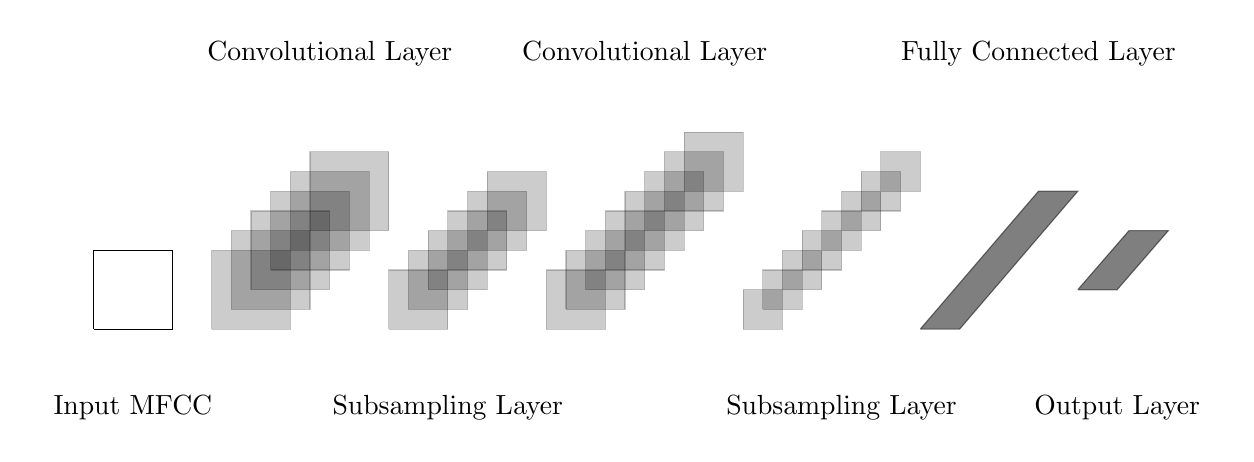
\begin{tikzpicture}
	\node at (0.5,-1){\begin{tabular}{c}Input MFCC\end{tabular}};
	
	\draw (0,0) -- (1,0) -- (1,1) -- (0,1) -- (0,0);
	
	\node at (3,3.5){\begin{tabular}{c}Convolutional Layer\end{tabular}};
	
	\draw[fill=black,opacity=0.2,draw=black] (2.75,1.25) -- (3.75,1.25) -- (3.75,2.25) -- (2.75,2.25) -- (2.75,1.25);
	\draw[fill=black,opacity=0.2,draw=black] (2.5,1) -- (3.5,1) -- (3.5,2) -- (2.5,2) -- (2.5,1);
	\draw[fill=black,opacity=0.2,draw=black] (2.25,0.75) -- (3.25,0.75) -- (3.25,1.75) -- (2.25,1.75) -- (2.25,0.75);
	\draw[fill=black,opacity=0.2,draw=black] (2,0.5) -- (3,0.5) -- (3,1.5) -- (2,1.5) -- (2,0.5);
	\draw[fill=black,opacity=0.2,draw=black] (1.75,0.25) -- (2.75,0.25) -- (2.75,1.25) -- (1.75,1.25) -- (1.75,0.25);
	\draw[fill=black,opacity=0.2,draw=black] (1.5,0) -- (2.5,0) -- (2.5,1) -- (1.5,1) -- (1.5,0);
	
	\node at (4.5,-1){\begin{tabular}{c}Subsampling Layer\end{tabular}};
	
	\draw[fill=black,opacity=0.2,draw=black] (5,1.25) -- (5.75,1.25) -- (5.75,2) -- (5,2) -- (5,1.25);
	\draw[fill=black,opacity=0.2,draw=black] (4.75,1) -- (5.5,1) -- (5.5,1.75) -- (4.75,1.75) -- (4.75,1);
	\draw[fill=black,opacity=0.2,draw=black] (4.5,0.75) -- (5.25,0.75) -- (5.25,1.5) -- (4.5,1.5) -- (4.5,0.75);
	\draw[fill=black,opacity=0.2,draw=black] (4.25,0.5) -- (5,0.5) -- (5,1.25) -- (4.25,1.25) -- (4.25,0.5);
	\draw[fill=black,opacity=0.2,draw=black] (4,0.25) -- (4.75,0.25) -- (4.75,1) -- (4,1) -- (4,0.25);
	\draw[fill=black,opacity=0.2,draw=black] (3.75,0) -- (4.5,0) -- (4.5,0.75) -- (3.75,0.75) -- (3.75,0);
	
	\node at (7,3.5){\begin{tabular}{c}Convolutional Layer\\\end{tabular}};
	
	\draw[fill=black,opacity=0.2,draw=black] (7.5,1.75) -- (8.25,1.75) -- (8.25,2.5) -- (7.5,2.5) -- (7.5,1.75);
	\draw[fill=black,opacity=0.2,draw=black] (7.25,1.5) -- (8,1.5) -- (8,2.25) -- (7.25,2.25) -- (7.25,1.5);
	\draw[fill=black,opacity=0.2,draw=black] (7,1.25) -- (7.75,1.25) -- (7.75,2) -- (7,2) -- (7,1.25);
	\draw[fill=black,opacity=0.2,draw=black] (6.75,1) -- (7.5,1) -- (7.5,1.75) -- (6.75,1.75) -- (6.75,1);
	\draw[fill=black,opacity=0.2,draw=black] (6.5,0.75) -- (7.25,0.75) -- (7.25,1.5) -- (6.5,1.5) -- (6.5,0.75);
	\draw[fill=black,opacity=0.2,draw=black] (6.25,0.5) -- (7,0.5) -- (7,1.25) -- (6.25,1.25) -- (6.25,0.5);
	\draw[fill=black,opacity=0.2,draw=black] (6,0.25) -- (6.75,0.25) -- (6.75,1) -- (6,1) -- (6,0.25);
	\draw[fill=black,opacity=0.2,draw=black] (5.75,0) -- (6.5,0) -- (6.5,0.75) -- (5.75,0.75) -- (5.75,0);
	
	\node at (9.5,-1){\begin{tabular}{c}Subsampling Layer\end{tabular}};
	
	\draw[fill=black,opacity=0.2,draw=black] (10,1.75) -- (10.5,1.75) -- (10.5,2.25) -- (10,2.25) -- (10,1.75);
	\draw[fill=black,opacity=0.2,draw=black] (9.75,1.5) -- (10.25,1.5) -- (10.25,2) -- (9.75,2) -- (9.75,1.5);
	\draw[fill=black,opacity=0.2,draw=black] (9.5,1.25) -- (10,1.25) -- (10,1.75) -- (9.5,1.75) -- (9.5,1.25);
	\draw[fill=black,opacity=0.2,draw=black] (9.25,1) -- (9.75,1) -- (9.75,1.5) -- (9.25,1.5) -- (9.25,1);
	\draw[fill=black,opacity=0.2,draw=black] (9,0.75) -- (9.5,0.75) -- (9.5,1.25) -- (9,1.25) -- (9,0.75);
	\draw[fill=black,opacity=0.2,draw=black] (8.75,0.5) -- (9.25,0.5) -- (9.25,1) -- (8.75,1) -- (8.75,0.5);
	\draw[fill=black,opacity=0.2,draw=black] (8.5,0.25) -- (9,0.25) -- (9,0.75) -- (8.5,0.75) -- (8.5,0.25);
	\draw[fill=black,opacity=0.2,draw=black] (8.25,0) -- (8.75,0) -- (8.75,0.5) -- (8.25,0.5) -- (8.25,0);
	
	\node at (12,3.5){\begin{tabular}{c}Fully Connected Layer\end{tabular}};
	
	\draw[fill=black,draw=black,opacity=0.5] (10.5,0) -- (11,0) -- (12.5,1.75) -- (12,1.75) -- (10.5,0);
	
	\node at (13,-1){\begin{tabular}{c}Output Layer \end{tabular}};
	
	\draw[fill=black,draw=black,opacity=0.5] (12.5,0.5) -- (13,0.5) -- (13.65,1.25) -- (13.15,1.25) -- (12.5,0.5);
	\end{tikzpicture}
	\caption[Typical convolutional neural network architecture.]{Typical convolutional neural network architecture.}
	\label{fig:tradCNN}
\end{figure*}
\begin{figure}[htp]
	\centering
	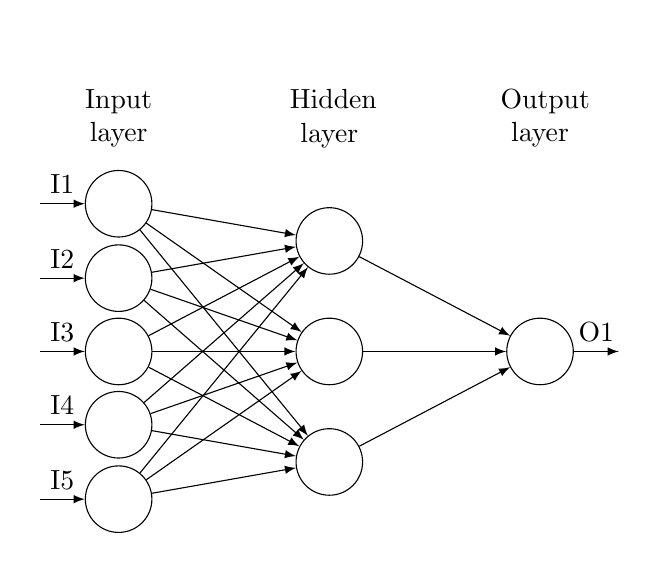
\begin{tikzpicture}[
	plain/.style={
		draw=none,
		fill=none,
	},
	net/.style={
		matrix of nodes,
		nodes={
			draw,
			circle,
			inner sep=8.5pt
		},
		nodes in empty cells,
		column sep=0.6cm,
		row sep=-11pt
	},
	>=latex
	]
	\matrix[net] (mat)
	{
		|[plain]| \parbox{1cm}{\centering Input\\layer} & |[plain]| \parbox{1cm}{\centering Hidden\\layer} & |[plain]| \parbox{1cm}{\centering Output\\layer} \\
		& |[plain]| \\
		|[plain]| & \\
		& |[plain]| \\
		|[plain]| & |[plain]| \\
		& & \\
		|[plain]| & |[plain]| \\
		& |[plain]| \\
		|[plain]| & \\
		& |[plain]| \\
	};
	\foreach \ai [count=\mi ]in {2,4,...,10}
	\draw[<-] (mat-\ai-1) -- node[above] {I\mi} +(-1cm,0);
	\foreach \ai in {2,4,...,10}
	{\foreach \aii in {3,6,9}
		\draw[->] (mat-\ai-1) -- (mat-\aii-2);
	}
	\foreach \ai in {3,6,9}
	\draw[->] (mat-\ai-2) -- (mat-6-3);
	\draw[->] (mat-6-3) -- node[above] {O1} +(1cm,0);
	\end{tikzpicture}
	
	\caption{Diagram of a generalised deep neural network.}
	\label{fig_m_3}
\end{figure}
\tikzset{%
	every neuron/.style={
		circle,
		draw,
		minimum size=1cm
	},
	neuron missing/.style={
		draw=none, 
		scale=4,
		text height=0.333cm,
		execute at begin node=\color{black}$\vdots$
	},
}
\def\layersep{2.5cm}



% Number of hidden layers chosen??


\subsection{Output}
Once put through the neural network, an ID will be outputted corresponding to one of the four emotions analysed. A look-up will be performed on this ID and the emotion will be displayed on the user interface, detailed in section~\ref{sec:ui}.

\subsection{User Interface}\label{sec:ui}
A simple user interface will be developed using Python's graphics library, TKinter. The interface will allow for users to start a 2~second voice recording. The recording will then be converted, input to the trained network and the emotional output will be displayed.

\subsection{Training and Testing Data}\label{sec:traintest}
Data gathered (through speech recordings and internet samples) will be separated into three groups, being data used for training, data used for testing and data used for validation. The training data is used to make the system accustomed to the required model and make the designed system respond as accurately to the desired outcome as possible. The validation dataset is used to tune the hyper-parameter of the model while also evaluating the system on it's initial training. The testing data is now used to check the final model along with it's results \cite{train}.

It is imperative that the dataset used for training be large, as through the inputs given the network will be 'taught' how to differentiate between different emotions and the more samples fed in at this stage, the higher the systems accuracy will be. Similarly, a large number of inputs should be used for test and validation databases in order to ensure accuracy in the system's success specifications.

In order to take these factors into account, a recommended 80\%  of data collected will be used for training and the remaining 20\% for testing, a ratio implemented in~\cite{RGB}
The data obtained from volunteers will be recorded in a sound proof room and then again with a noisy background where the first instance will be used to train the system and the latter to test it.

\hfill\\
In addition to a singular model trained, combinations of filters and topologies will be shuffled around and their outputs compared, for example the MLP network with no filters applied to inputs, the CNN with one filter applied and the MLP with all developed filters applied. Finally, accuracy between the English and Afrikaans systems will be compared.

\section{Project Management}\label{sec:management}
Throughout the duration of the project, the partners will be in contact with each other regarding their progress or any other obstacles which they may face. In addition, at least one weekly face-to-face meeting will be held between the partners and project supervisor.

Project files will be housed on a private GitHub repository.
The subsections following will outline how the project components listed in section Approach  will be divided and the estimated time to be taken for each. In addition, a gantt chart of the proposed project timeline is illustrated in appendix~\ref{sec:gantt}, and its work breakdown structure in appendix~\ref{sec:wbs}.

It is important to note that in project planning, each aspect was timed in order to leave a week free in case of delays experienced during development.

%~~~~~~~~~~~~~~~~~~~~~~~~~~~~~~~~~~~~~~~~~~~~~~~~~~~~~~~~~~~~~~~~~~~~~~~~~~~~~~~~~~~~~~~~~~~~~

\newcolumntype{R}[1]{>{\raggedright\let\newline\\\arraybackslash\hspace{0pt}}m{#1}}

\subsection{Project Initiation}
At the start of the project technical,  set-up is necessary. These tasks are detailed in table~\ref{table:init} 

\begin{table}[h]
	\caption{Table listing initiation task details.}
	\begin{tabular}{|R{3.3cm}ll|}
		\hline
		\multicolumn{1}{|l}{Task} & \multicolumn{1}{l}{Duration} & Group Member \\ \hline
		Setup GitHub repo &       0 days            &   S.S. Berkowitz           \\
Install Python 3.5   &        0.25 days       &     Collective   \\
		Install TensorFlow &      0.25 days       &     Collective \\
		\hline
	\end{tabular}
	\label{table:init}
\end{table}

\textbf{Resources required:} Git

%~~~~~~~~~~~~~~~~~~~~~~~~~~~~~~~~~~~~~~~~~~~~~~~~~~~~~~~~~~~~~~~~~~~~~~~~~~~~~~~~~~~~~~~~~~~~~

\subsection{Data Collection}
Collection of data will be done through utilising both online sources and recordings made in person and have been listed in the table items below. A full two week period will be used for sourcing and separating data, which will be done in parallel and organised as it is collected. A full breakdown of the tasks is shown in table~\ref{table:data}. Organising of data will also include splitting it into 2 second files.
\begin{table}[h]
	\caption{Table listing data collection task details.}
	\begin{tabular}{|R{3.3cm}ll|}
		\hline
		\multicolumn{1}{|l}{Task} & \multicolumn{1}{l}{Duration} & Group Member \\ \hline
		Setup recording equipment &       0.5 days            &   S.S. Berkowitz           \\
		Collect data via recordings   &        9 days       &     Collective   \\
		Collect data via online sources &      9 days       &     Collective \\
		Organise data &                9 days     &   Collective   \\
		\hline
	\end{tabular}
	\label{table:data}
\end{table}

\textbf{Resources required:} Microphone, Recording application, access to soundproof chamber

%~~~~~~~~~~~~~~~~~~~~~~~~~~~~~~~~~~~~~~~~~~~~~~~~~~~~~~~~~~~~~~~~~~~~~~~~~~~~~~~~~~~~~~~~~~~~~

\subsection{Signal Enhancement}

The signal enhancement phase will include the implementation of the four noise cancellation algorithms and applying them to the datasets. Each partner will be responsible for two separate algorithms and applying them to the collected data. These tasks will be implemented in parallel and their details are listed in table~\ref{table:enhancement}.

\begin{table}[h]
	\caption{Table listing signal enhancement task details.}
	\begin{tabular}{|R{3.3cm}ll|}
		\hline
		\multicolumn{1}{|l}{Task} & \multicolumn{1}{l}{Duration} & Group Member \\ \hline
		Implementation of Algorithm 1 &       2 days            &   S.S. Berkowitz           \\
		Implementation of Algorithm 2 &       2 days            &   A. Pathania          \\
		Implementation of Algorithm 3 &       2 days            &   S.S. Berkowitz           \\
		Implementation of Algorithm 4 &       2 days            &   A. Pathania           \\
		Application of alorithms 1 \& 3 &                1 days     &   S.S. Berkowitz   \\
		Application of alorithms 2 \& 4 &                1 days     &   A. Pathania   \\
		\hline
	\end{tabular}
	\label{table:enhancement}
\end{table}

\textbf{Resources required:} Python 3.5


\subsection{Signal Classification}

The two  partners will work in parallel developing the two neural network topologies for the project, details of which can be seen in table~\ref{table:class}

\begin{table}[h]
	\caption{Table listing signal classification task details.}
	\begin{tabular}{|R{3.3cm}ll|}
		\hline
		\multicolumn{1}{|l}{Task} & \multicolumn{1}{l}{Duration} & Group Member \\ \hline
		MLP code design &       1 days            &   A. Pathania           \\
		Convolution Neural Network code design &       1 days            &   S.S. Berkowitz         \\
		MLP code implementation &       4 days            &   A. Pathania            \\
		Convolution Neural Network code implementation &       4 days            &   S.S. Berkowitz          \\
		\hline
	\end{tabular}
	\label{table:class}
\end{table}


\textbf{Resources required:} Python 3.5, TensorFlow

\subsection{User Interface}

The final week of the project will focus on the development of a live integration and a user interface. These tasks are separated in table~\ref{table:ui}.

\begin{table}[h]
	\caption{Table listing signal classification task details.}
	\begin{tabular}{|R{3.3cm}ll|}
		\hline
		\multicolumn{1}{|l}{Task} & \multicolumn{1}{l}{Duration} & Group Member \\ \hline
		Python recording \& conversion &       2 days            &   A. Pathania           \\
		I/O integration &       2 days            &   A. Pathania           \\
		User interface &      4  days            &   S.S. Berkowitz         \\
		\hline
	\end{tabular}
	\label{table:ui}
\end{table}

\textbf{Resources required:} Python, TKinter

\section{RISKS AND THEIR MITIGATIONS}\label{sec:risks}
\subsection{Data Security}

The researchers have access to the voices of several individuals from various sources. This data can be subjected to misuse as it can be stolen from the computers used for the study and cloned to hack into the individual's computer.This  personal information taken out of context can lead to data breach and pose a threat to the individual's privacy.

The method of mitigation in this case is to securely keep the voice samples on the researchers computers in a password protected file and destroy these samples as soon as the project finishes, which is after six weeks of the project commencement. This data at no point in time will be shared by any third party candidate for any use.This way the cloning of the samples can be protected. 
\subsection{Ethical Issues}
The access of any individual's personal belonging is a matter of ethical interest.  The researchers could take data from students around campus and later use it to for means that are not included in their study.This would expose the private information of volunteers to the public. 

The methods of mitigation for this risk is as follows:
The participants are all volunteers and are willingly contributing to the study.They will be provided by an information sheet to explain to the them the process of the study and they can leave the study at any given time if the wish to. The will be given a piece of literature to speak and will thus not provide any personal information. An ethics clearance is applied by the researchers to gather this data from the ethics committee of the University of Witwatersrand and no data acquisition will be started without an acceptance letter from the committee.

\subsection{Inaccurate Results}
The system is trained with data either obtained from online sources or recorded voices of students willing to participate in the study. Both data sets are prone to a number of background noises or channel distortion which will interfere in the proper training of the system. If the system is not properly trained it might end up giving inaccurate results  

The proper mitigation for this system includes using the online data from sources which specify that the data has been used in speech recognition systems and hence has been recorded in a low noise environment with good equipments.The data recording done by the researchers should be performed in a soundproof chamber to minimize the distortion in the recordings. T The system is expected to give an accuracy of 50\%. The system then undergoes through tests which will be run on the data to see if the desired outcome is achieved.

\subsection{Intellectual Property Risks}
Intellectual property risks often causes trouble for innovators or researchers trying to build something new in software. As patenting would only apply to their code implementation and not their design they are at risk.

In the case of Machine Learning this risk is not as evident as it is not as dependent on code implementation as much as the amount of data that is used to train the developed models. Therefore, a third party is less disposed to stealing the resultant system which will have an accuracy dependant on how well the system is trained with gathered data.

\section{Social Impacts}\label{sec:social}
With the ever-changing global economic status, the average person's lifestyle is affected, where they are constantly looking for their best suited source for goods and services~\cite{airelevant}. As such, businesses need to look for new innovation in order to stay relevant to customers, customer service being a main aspect. 

Artificial intelligence (and emotion recognition within it) has become ever more relevant within this field with the automation of the customer-provider experience. Employing such technologies provide efficiency in customer's time, lengthens hours that the provider can be contacted, as well as assists in providing answers going beyond a script or set of questions a human is trained to answer as machines formulate their own solutions with the assistance of deep learning~\cite{airelevant}. The implementation of the above not only causes a better customer experience, but also has a positive impact on the business itself as well as the local economy by keeping customers' interests local~\cite{airelevant}.

With the positive impacts this technology has on an employer, it also provides a negative one to the employee. Due to the increase in technological assistance, a Forrester study estimated that 25\% of jobs will be at risk by 2019~\cite{chatbot}. As such, studies in AI and human understanding can have a negative effect and changes, on the part of workers, should be made in order to keep up with the current job market.


\section{CONCLUSION}\label{sec:conc}
This report discusses the relevance of Artificial Intelligence and more specifically emotion recognition from speech. It introduces the plan for implementing a project which is able to identify happiness, sadness, fear and anger from human speech of both English and Afrikaans speakers. The report further discusses the details of the methodology used for implementing the aforementioned system. Adaptive filters are used to cancel the background noise since they adjust their parameters according to the requirement of the environment, followed by MFCC being used to recognise the relevant aspects of the signal to make them suitable input for a neural network. The Machine Learning algorithms, MLP and CNN, finally give an output which states the emotion detected. The expected accuracy based on reviewed literature is above 50\%. The project has a six weeks deadline within which the researchers are expected to collect data, process it, train the system and finally validate its functionality. The report further discusses data breaches and other risks which the study may impose during it's execution, along with mitigations to be taken on each and the social impact of the study on society.



\vspace{7pt}
\bibliographystyle{ieeetr}
\begin{thebibliography}{1}
	
	\bibitem{chatbot} Heek, N.F. {\em How Chatbots are Killing Jobs and Creating New Ones}, 2017. https://venturebeat.com/2017/06/18/how-chatbots-are-killing-jobs-and-creating-new-ones/ [Last accessed: 15-07-2018]
	
	\bibitem{tensorIntro} Shaikh, F. {\em An Introduction to Implementing Neural Networks using TensorFlow}, 2016. https://www.analyticsvidhya.com/blog/2016/10/an-introduction-to-implementing-neural-networks-using-tensorflow/ [Last accessed: 13-07-2018]
	
	
	\bibitem{fearMLP} Ram, R., Palo H.K., Mohanty, M.N. {\em Recognition of Fear from Speeach using Adaptive Algorithm with MLP Classifier} ICCPCT, 2016.
	
	\bibitem{RGB} Stolar, M.N., Lech, M., Bolia, R.S, Skinner, M. {\em Real Time Speech Emotion Recognition Using RGB Image Classification and Transfer Learning} School of Engineering, RMIT University, 2017.
	
		
	\bibitem{echo} Hamidia, M., Amrouche, A. {\em Improved Variable Step-Size Adaptive Filtering Algorithm or Acoustic Echo Cancellation} USTHB Faculty of Electronics and Computer Science, 2015.
	
	
		\bibitem{recordingFreq} Hill, Andrew R. {\em Analysis of Voice Recordings Made Using "Voice Memos" Application for iOS} University of Colorado, Denver, p.28, 2014.
		
			\bibitem{FAP} Steven L. G., Tavathia A. {\em THE FAST AFFINE PROJECTION ALGORITHM} ,Acoustics Research Department
		AT\&T Bell Laboratories.
		
		
		
		\bibitem{MFCC-1}  Shrawankar  U., Thakare  V. {\em TECHNIQUES FOR FEATURE EXTRACTION IN SPEECH
			RECOGNITION SYSTEM: A COMPARATIVE STUDY} ,(Computer Science \& Engg.), SGB Amravati University .
	
	\bibitem{airelevant} Bansal, S. {\em Why is Artificial Intellegence (AI) Relevant Today?}, 2017. https://www.linkedin.com/pulse/why-artificial-intelligence-ai-relevant-today-sanjiv-bansal [Last accessed: 15-07-2018]
	
	
	
	% 8
	\bibitem{MFCC-3} Gevaert W., Tsenov G., Mladenov V. {\em Neural Networks used for Speech Recognition } ,JOURNAL OF AUTOMATIC CONTROL, UNIVERSITY OF BELGRADE,2010.
	

	
	
	\bibitem{RLS}Singh, K., Gu Y. {\em Speech Enhancement Based On Noise Reduction} ,Electrical Engineering Department, University Of Rochester, 2016.
	

	% 10
	\bibitem{MFCC-2}  Wyse  L. {\em Audio spectrogram representations for processing with Convolutional Neural Networks} ,National University of Singapore, January 2017.
	
	
	
	\bibitem{CNN} Sainath, T.N., Parada, C. {\em Convolutional Neural Networks for Small-footprint Keyword Spotting}, Google Inc., New York, 2015.
	
	
	
	\bibitem{train} TARANG SHAH {\em Train, Validation and Test Sets}Dec 2017. Available at : http://tarangshah.com/blog/2017-12-03/train-validation-and-test-sets/ [Last Accessed on : 15 July 2018]
	
	
	
\end{thebibliography}

\onecolumn

\begin{appendix}
	\section{Work Breakdown Structure}\label{sec:wbs}
	The proposed work breakdown structure for the project follows:
	\hfill\\
	\begin{rotate}{270}
		\noindent\rule{1.75cm}{0.4pt}
		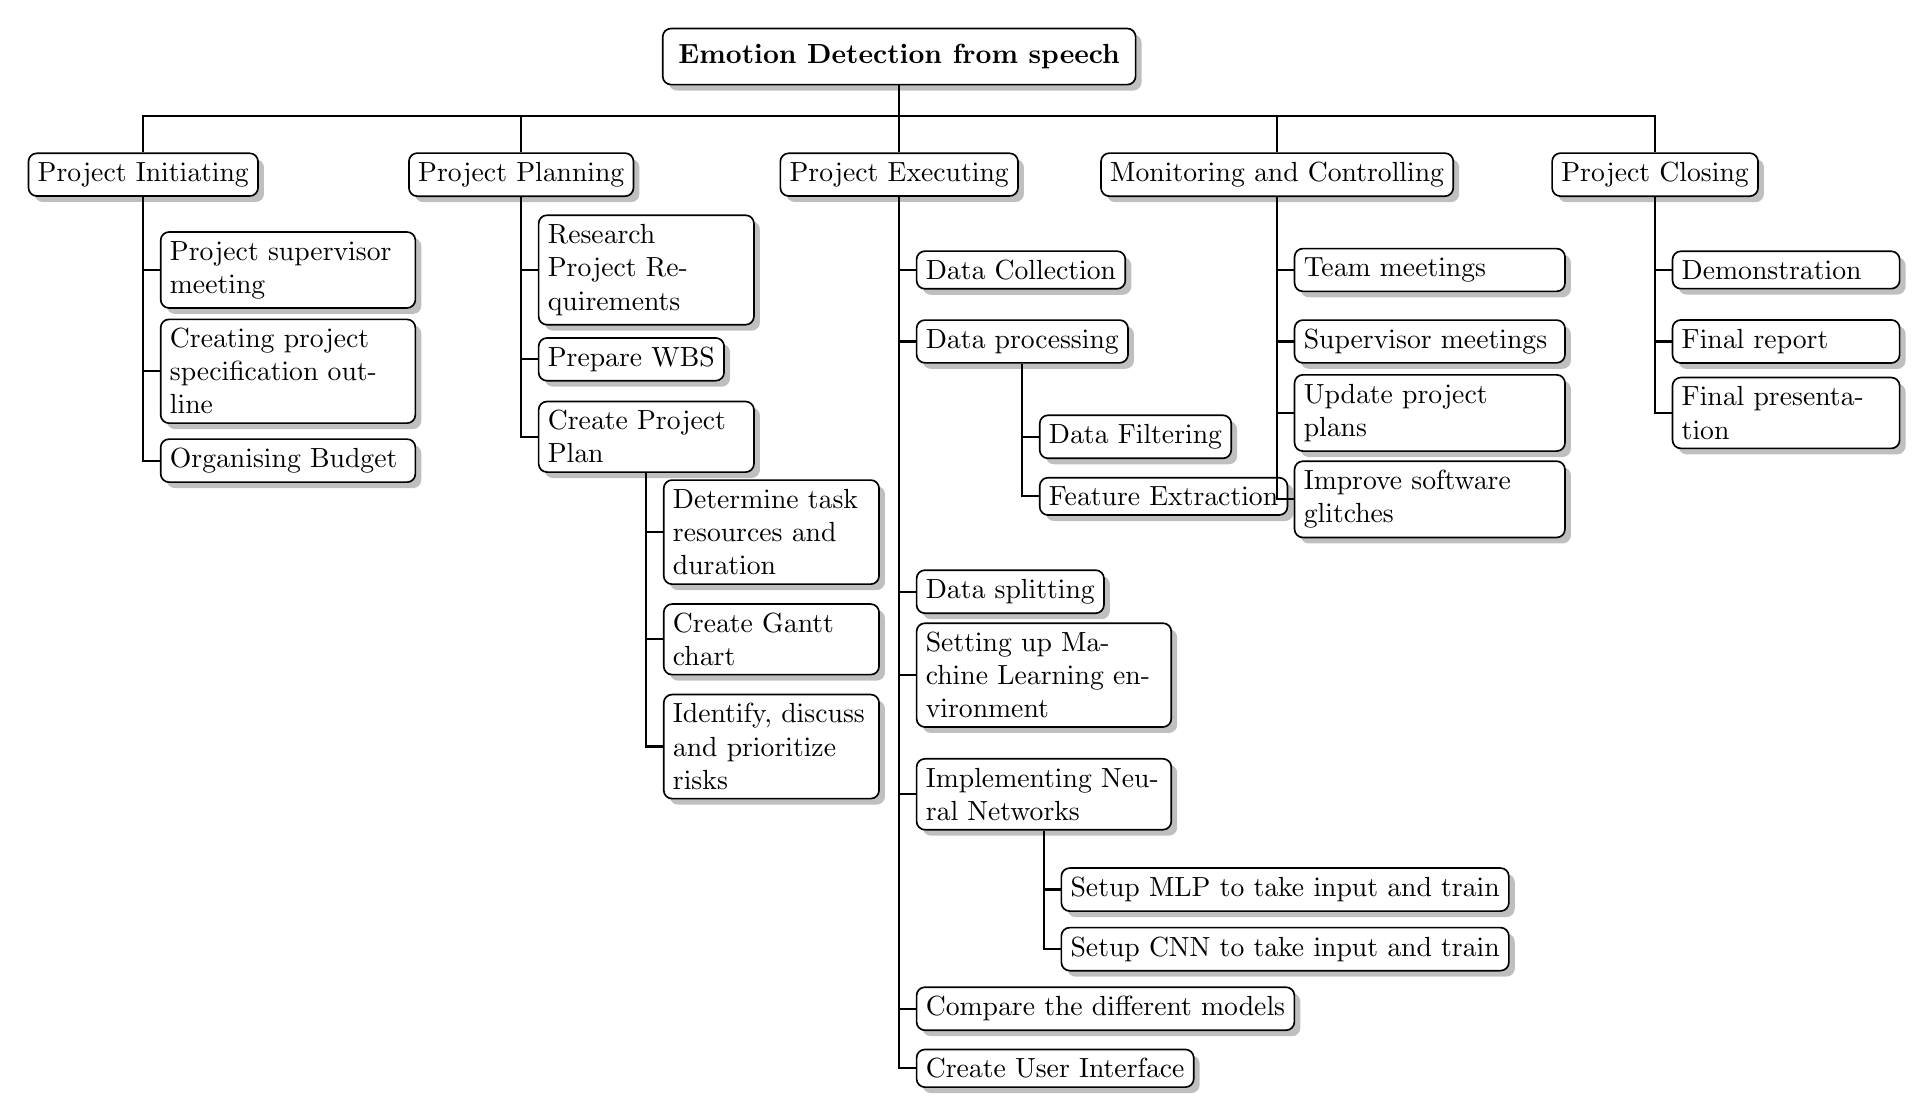
\begin{tikzpicture}[
		every node/.style = {draw, rounded corners=3pt, semithick, drop shadow},
		ROOT/.style = {top color=white!60, bottom color=white!60!,
			inner sep=2mm, text=black, font=\bfseries},
		L1/.style = {fill=white!20},
		L2/.style = {fill=white!30},
		L3/.style = {fill=white!30, grow=down, xshift=0.3em, anchor=west, 
			edge from parent path={(\tikzparentnode.south) |- (\tikzchildnode.west)}},
		edge from parent/.style = {draw, thick},
		LD/.style = {level distance=#1ex},
		LD1/.style = {level distance=8ex},
		LD2/.style = {level distance=18ex},
		LD3/.style = {level distance=26ex},
		% LD4/.style = {level distance=30ex},
		level 1/.style = {sibling distance=48mm}
		]
		
		% Parents
		\node[ROOT] {Emotion Detection from speech}
		[edge from parent fork down]
		child{node[L2] {Project Initiating}
			child[L3,LD1]   {node[L3, text width=3cm]   {Project supervisor meeting}}
			child[L3,LD=16.5]  {node[L3, text width=3cm]   {Creating project specification outline}}
			child[L3,LD=24]   {node[L3, text width=3cm]   {Organising Budget}}
		}
		child{node[L2] {Project Planning}
			child[L3,LD1]  {node[L3, text width=2.5cm]   {Research Project Requirements}}
			child[L3,LD=15.5]  {node[L3]   {Prepare WBS}}
			child[L3,LD=22]  {node[L3, text width=2.5cm]   {Create Project Plan}
				child[L3,LD1] {node[L3, text width=2.5cm]   {Determine task resources and duration}}
				child[L3,LD=17] {node[L3, text width=2.5cm]   {Create Gantt chart}}
				child[L3,LD3] {node[L3, text width=2.5cm]   {Identify, discuss and prioritize risks}}}
		}
		child {node[L2] {Project Executing}
			child[L3,LD1] {node[L3]   {Data Collection}}
			child[L3,LD=14] {node[L3]   {Data processing}
				child[L3,LD1] {node[L3]   {Data Filtering}}
				child[L3,LD=13] {node[L3,fill=white!30]   {Feature Extraction}} 
			}     
			child[L3,LD=35]  {node[L3]   {Data splitting}}
			child[L3,LD=42]  {node[L3, text width=3cm]   {Setting up Machine Learning environment}}
			child[L3,LD=52]  {node[L3, text width=3cm]   {Implementing Neural Networks}
				child[L3,LD1] {node[L3,fill=white!30]   {Setup MLP to take input and train}} 
				child[L3,LD=13] {node[L3,fill=white!30]   {Setup CNN to take input and train}} 
			}
			child[L3,LD=70]  {node[L3]   {Compare the different models}}
			child[L3,LD=75]  {node[L3]   {Create User Interface}}
		}
		child {node[L2] {Monitoring and Controlling}
			child[L3,LD1] {node[L3,text width=3.2cm]   {Team meetings}}
			child[L3,LD=14] {node[L3,text width=3.2cm]   {Supervisor meetings}}
			child[L3,LD=20] {node[L3,text width=3.2cm]   {Update project plans}}            
			child[L3,LD=27.25] {node[L3,text width=3.2cm]   {Improve software glitches}}
		}    
		child {node[L2] {Project Closing}
			child[L3,LD1] {node[L3, text width=2.65cm]   {Demonstration}}
			child[L3,LD=14] {node[L3, text width=2.65cm]   {Final report}}     
			child[L3,LD=20]  {node[L3, text width=2.65cm]   {Final presentation}}
		};
		\end{tikzpicture}
	\end{rotate}
	
\newpage
	\section{Gantt Chart}\label{sec:gantt}
The gantt chart of the proposed project timeline follows:
%	\begin{landscape}
		\ganttset{%
			calendar week text={%
				\pgfcalendarmonthshortname{\startmonth}~\startday, \startyear%
			}%
		}
		\newganttchartelement*{sresource}{
			sresource/.style={},
			inline=true,
			sresource inline label node/.style={anchor=west,font=\bfseries\itshape\color{purple}},
			sresource left shift=0ex,
			sresource right shift=0ex
		}
		\newganttchartelement*{aresource}{
			aresource/.style={},
			inline=true,
			aresource inline label node/.style={anchor=west,font=\bfseries\itshape\color{blue}},
			aresource left shift=0ex,
			aresource right shift=0ex
		}
		\newganttchartelement*{cresource}{
			cresource/.style={},
			inline=true,
			cresource inline label node/.style={anchor=west,font=\bfseries\itshape\color{green}},
			cresource left shift=0ex,
			cresource right shift=0ex
		}
	
	
	\begin{flushleft}
		\begin{rotate}{270}
			
		\begin{ganttchart}[
			hgrid,
			vgrid,
			x unit=4mm,
			time slot format=isodate
			]{2018-07-16}{2018-08-24}
			\gantttitlecalendar{year, month=name, day} \\
			\ganttsresource{S. Berkowitz}{2018-07-17}
			\ganttbar[inline=false]{Set-up Github Repository}{2018-07-16}{2018-07-16} \\
			\ganttcresource{Collective}{2018-07-17}
			\ganttbar[inline=false]{Verify Correct Python Installation}{2018-07-16}{2018-07-16} \\
			\ganttcresource{Collective}{2018-07-17}
			\ganttbar[inline=false]{Verify Correct TensorFlow Installation}{2018-07-16}{2018-07-16} \\
			\ganttsresource{S. Berkowitz}{2018-07-18}
			\ganttbar[inline=false]{Setup recording equipment}{2018-07-17}{2018-07-17} \\
			\ganttcresource{Collective}{2018-07-28}
			\ganttbar[inline=false]{Collect data via recordings}{2018-07-18}{2018-07-27} \\
			\ganttcresource{Collective}{2018-07-28}
			\ganttbar[inline=false]{Collect data via online sources}{2018-07-17}{2018-07-27} \\
			\ganttcresource{Collective}{2018-07-28}
			\ganttbar[inline=false]{Organise data collected}{2018-07-17}{2018-07-27} \\
			\ganttsresource{S. Berkowitz}{2018-08-01}
			\ganttbar[inline=false]{Implement filter 1}{2018-07-30}{2018-07-31} \\
			\ganttaresource{A. Pathania}{2018-08-01}
			\ganttbar[inline=false]{Implement filter 2}{2018-07-30}{2018-07-31} \\
			\ganttsresource{S. Berkowitz}{2018-08-03}
			\ganttbar[inline=false]{Implement filter 3}{2018-08-01}{2018-08-02} \\
			\ganttaresource{A. Pathania}{2018-08-03}
			\ganttbar[inline=false]{Implement filter 4}{2018-08-01}{2018-08-02} \\
			\ganttsresource{S. Berkowitz}{2018-08-04}
			\ganttbar[inline=false]{Application of filters 1 \& 3}{2018-08-03}{2018-08-03} \\
			\ganttaresource{A. Pathania}{2018-08-04}
			\ganttbar[inline=false]{Application of filters 2 \& 4}{2018-08-03}{2018-08-03} \\
			\ganttlink{elem5}{elem7}
			\ganttlink{elem7}{elem9}
			\ganttlink{elem5}{elem11}
			\ganttlink{elem9}{elem15}
			\ganttlink{elem11}{elem15}
			\ganttlink{elem13}{elem15}
			\ganttlink{elem13}{elem17}
			\ganttlink{elem17}{elem19}
			\ganttlink{elem19}{elem23}
			\ganttlink{elem23}{elem25}
			
			%           \ganttbar{MLP code design}{2018-08-06}{2018-08-06} \\
			%           \ganttbar{CNN code design}{2018-08-06}{2018-08-06} \\
			%           \ganttbar{MLP code implementation}{2018-08-07}{2018-08-10} \\
			%           \ganttbar{CNN code implementation}{2018-08-07}{2018-08-10} \\
			%           \ganttbar{In-app recording code}{2018-08-13}{2018-08-14} \\
			%           \ganttbar{I\\O integration}{2018-08-15}{2018-08-16} \\
			%           \ganttbar{User interface development}{2018-08-13}{2018-08-16} \\
		\end{ganttchart}
	
	\end{rotate}
\end{flushleft}
	

\newpage
\begin{rotate}{270}
		\begin{ganttchart}[
			hgrid,
			vgrid,
			x unit=4mm,
			time slot format=isodate
			]{2018-07-16}{2018-08-24}
			\gantttitlecalendar{year, month=name, day} \\
			%           \ganttbar{Set-up Github Repository}{2018-07-16}{2018-07-16} \\
			%           \ganttbar{Verify Correct Python Installation}{2018-07-16}{2018-07-16} \\
			%           \ganttbar{Verify Correct TensorFlow Installation}{2018-07-16}{2018-07-16} \\
			%           \ganttbar{Setup recording equipment}{2018-07-17}{2018-07-17} \\
			%           \ganttbar{Collect data via recordings}{2018-07-18}{2018-07-27} \\
			%           \ganttbar{Collect data via online sources}{2018-07-17}{2018-07-27} \\
			%           \ganttbar{Organise data collected}{2018-07-17}{2018-07-27} \\
			%           \ganttbar{Implement filter 1}{2018-07-30}{2018-07-31} \\
			%           \ganttbar{Implement filter 2}{2018-07-30}{2018-07-31} \\
			%           \ganttbar{Implement filter 3}{2018-08-01}{2018-08-02} \\
			%           \ganttbar{Implement filter 4}{2018-08-01}{2018-08-02} \\
			%           \ganttbar{Application of filters 1 \& 3}{2018-08-03}{2018-08-03} \\
			%           \ganttbar{Application of filters 2 \& 4}{2018-08-03}{2018-08-03} \\
			\ganttaresource{A. Pathania}{2018-08-07}
			\ganttbar[inline=false]{MLP code design}{2018-08-06}{2018-08-06} \\
			\ganttsresource{S. Berkowitz}{2018-08-07}
			\ganttbar[inline=false]{CNN code design}{2018-08-06}{2018-08-06} \\
			\ganttaresource{A. Pathania}{2018-08-11}
			\ganttbar[inline=false]{MLP code implementation}{2018-08-07}{2018-08-10} \\          		\ganttsresource{S. Berkowitz}{2018-08-11}
			\ganttbar[inline=false]{CNN code implementation}{2018-08-07}{2018-08-10} \\
			\ganttaresource{A. Pathania}{2018-08-15}
			\ganttbar[inline=false]{In-app recording code}{2018-08-13}{2018-08-14} \\
			\ganttaresource{A. Pathania}{2018-08-15}
			\ganttbar[inline=false]{I\\O integration}{2018-08-15}{2018-08-16} \\
			\ganttsresource{S. Berkowitz}{2018-08-17}
			\ganttbar[inline=false]{User interface development}{2018-08-13}{2018-08-16} \\
			
			
			\ganttlink{elem1}{elem3}          
			\ganttlink{elem3}{elem5}
			\ganttlink{elem5}{elem9}
			\ganttlink{elem9}{elem11}
			\ganttlink{elem7}{elem13}
			
		\end{ganttchart}
	\end{rotate}
		
%	\end{landscape}
	
	
\end{appendix} 	


\end{document}